% Section: Experiments
\section{Experiments} \label{sec:experiment}


%% First
\subsection{First Experiment}

\para{Dataset}
Our first experiment is conducted on a one-dimensional data as shown in Figure~\ref{fig:data1}. In this experiment, we have a 543-point training set ranging from $x = -32$ to $x = 14$, and we want to predict some 67-point test set ranging from $x = 14$ to $x = 21$.

\begin{figure}[htp]
\begin{minipage}[htp]{1\linewidth}
	\centering
  	\subfloat{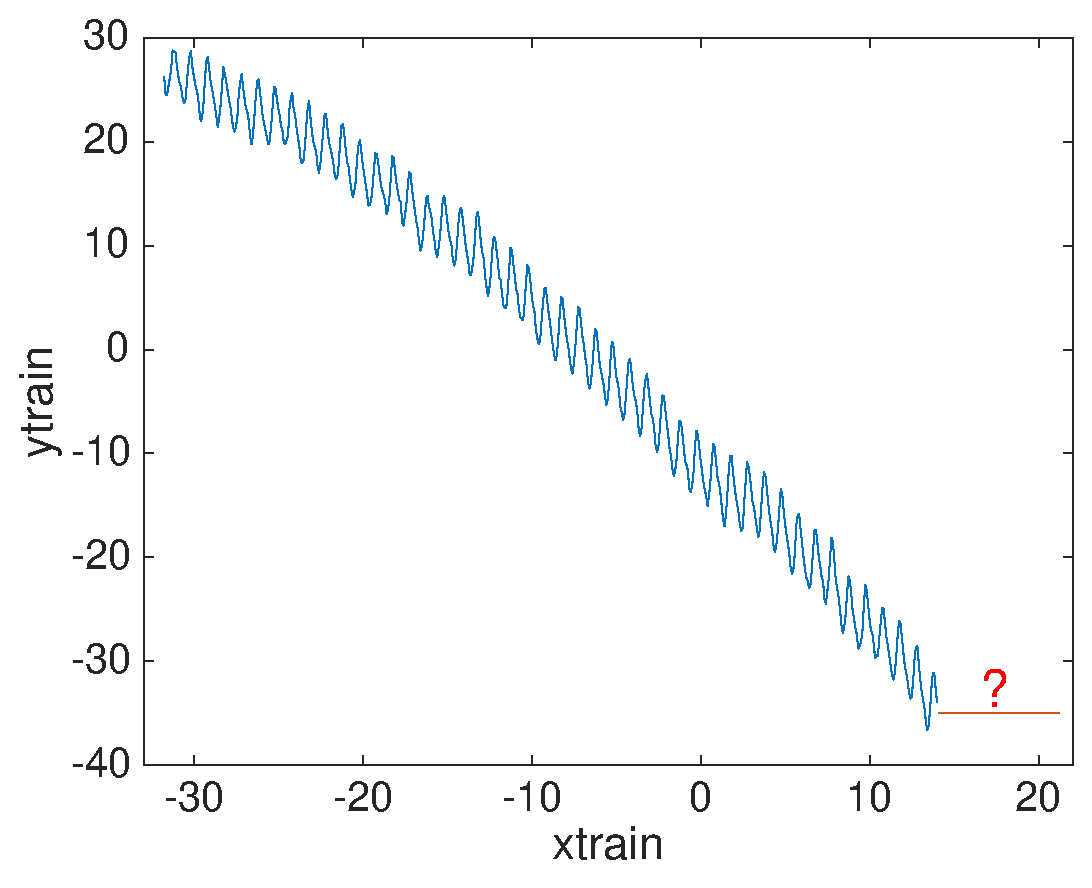
\includegraphics[width=0.7\textwidth]{figure/data1.eps}}
% \vspace{-0.1in}
\caption{A one-dimensional dataset}
\label{fig:data1} % FIG1
\end{minipage}
\vspace{-0.05in}
\end{figure}

\para{Auto Kernel Construction}
To better do this work, we use the Auto Construction Kernel method described in Section~\ref{sec:autokernel}.
By doing a lengthy greedy kernel construction procedure, we derive a compositional kernel:
\begin{equation}
LIN \times SE + SE \times ( PER + RQ )
\end{equation}

\begin{figure}[htp]
\begin{minipage}[htp]{1\linewidth}
	\centering
  	\subfloat{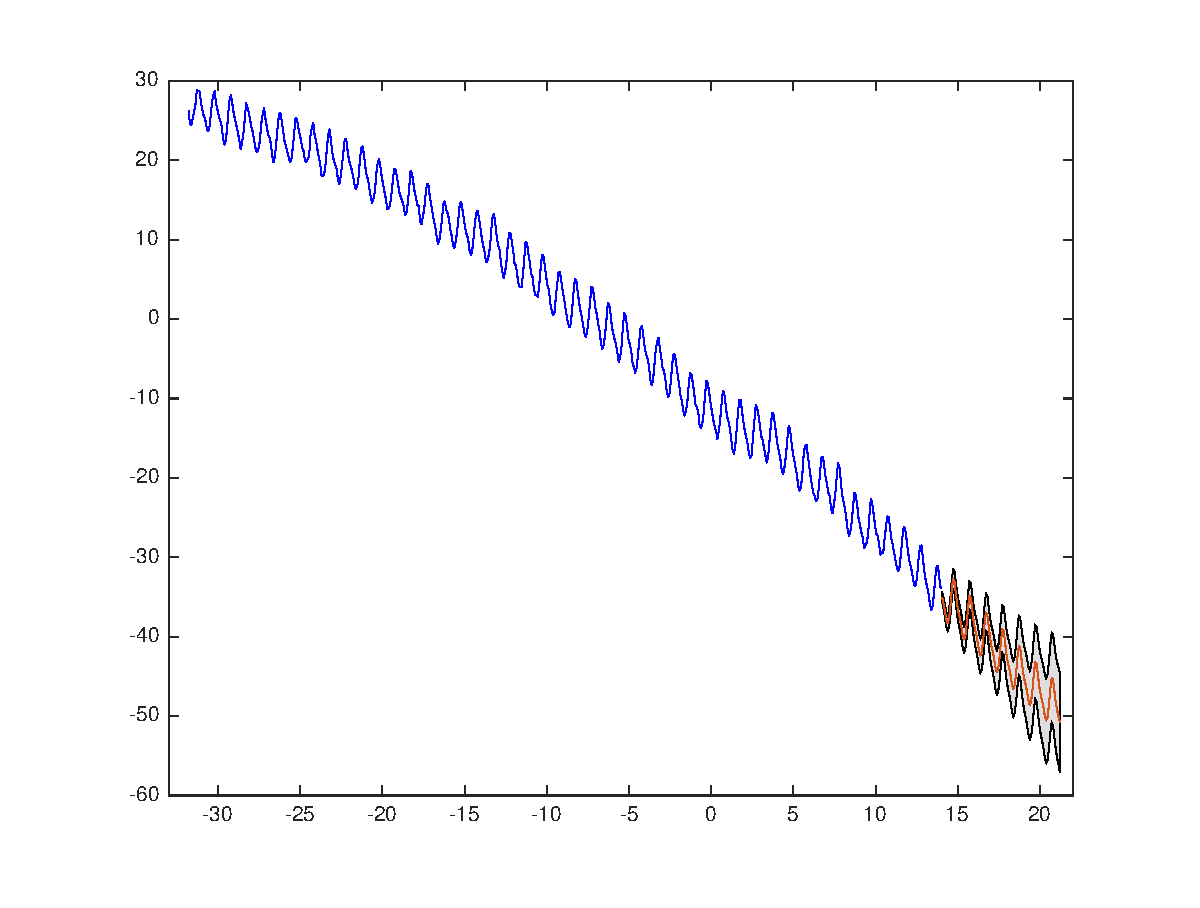
\includegraphics[width=0.8\textwidth]{figure/predict1.eps}}
% \vspace{-0.1in}
\caption{Prediction of the 1st dataset}
\label{fig:predict1} % FIG1
\end{minipage}
\vspace{-0.05in}
\end{figure}

\para{Result} 
And by using the \emph{Linear}, Mean Function \emph{Guassian} Likelihood function and the \emph{Exact} posterior probability.
(Note that we have also optimized the hyperparameters in all experiments.)
We predict the results as in Figure~\ref{fig:predict1}.
We could achieve an \textbf{MSE} of \textbf{0.2112} using this method. Given that the output data ranges from $-60~ to~30$, we believe that we have a satisfying result.



%% Second
\subsection{Second Experiment}

\begin{figure}[htp]
\begin{minipage}[htp]{1\linewidth}
	\centering
  	\subfloat{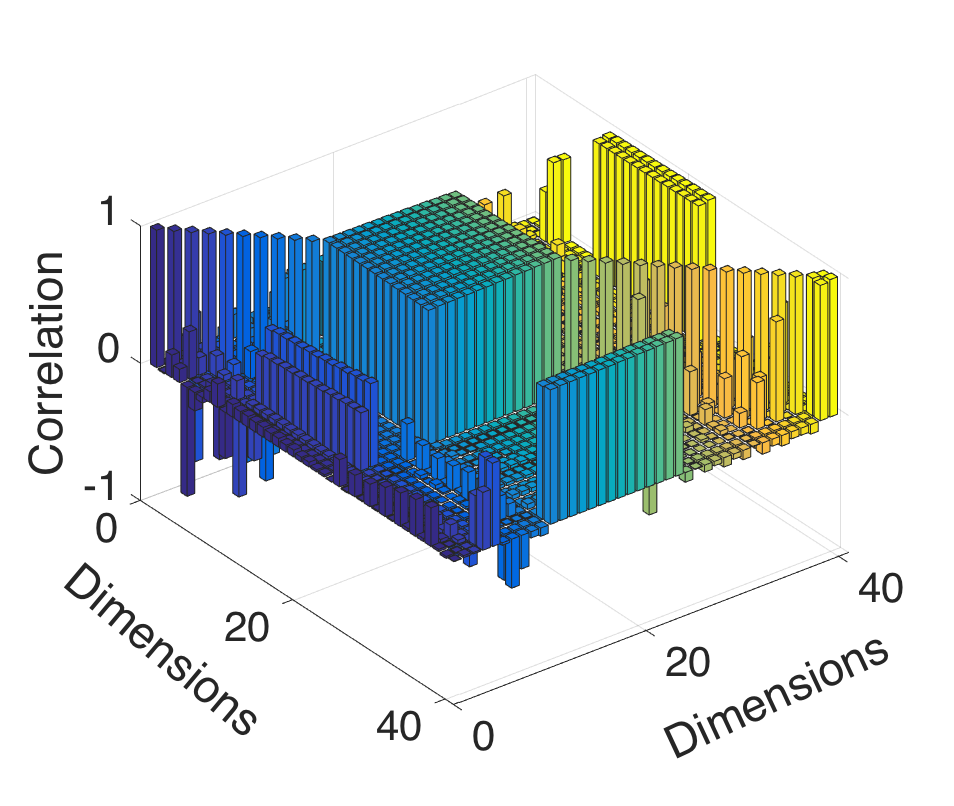
\includegraphics[width=0.9\textwidth]{figure/data2.eps}}
% \vspace{-0.1in}
\caption{Ailerons dataset, Correlation between each dimension of \textbf{x}. We can see that in the dimension set \{11:24, 39,40\}, variables are highly correlated with each other.}
\label{fig:data2}
\end{minipage}
\vspace{-0.05in}
\end{figure}

\para{Dataset}
The second dataset called \color{blue}\href{http://www.dcc.fc.up.pt/~ltorgo/Regression/ailerons.html}{\emph{Ailerons}}\color{black}\footnote{Available at \color{blue}\href{http://www.dcc.fc.up.pt/~ltorgo/Regression/ailerons.html}{www.dcc.fc.up.pt/~ltorgo/Regression/ailerons} \color{black}.}
is from the \emph{Experiments of Rui Camacho(rcamacho@garfield.fe.up.pt)}, it addresses a control problem of F16 aircraft. The goal is to predict the control action on the ailerons of the aircraft.
This dataset contains 40 attributes with a 10,000-point training set and a 3,750-point test set.

\para{Preprocessing}
Given a such high-dimensional dataset, we decide to first analyze the relationship between each dimension.
As shown in Figure~\ref{fig:data2}, we can see that actually 16 dimensions of the 40-dimensional \textbf{x} are highly correlated to each other (correlation > 0.96).
So reducing the dimension of this dataset is a probable way to reduce the complexity of the algorithm.
Thus, we do this procedure by ignoring the \{12:24, 39,40\}th dimensions, which are all highly correlated with the 11th dimension. And we consequently derive a 25-dimensional set with the \{1:11, 25:38\}th dimensions. \\

As follows, we are going to use two respective methods, the first one is through the auto construction of kernels, the second one is through the characteristics of an additive kernel as described in Section~\ref{sec:addGauss}.

%%% ABCD
\subsubsection{Auto Kernel Construction} \label{sec:pred2auto}
By conducting a greedy kernel search as in the previous experiment, we get a desired kernel function: \emph{SE}.
We hereby use this kernel and test its performance on different \emph{Likelihood Functions} and \emph{Inference Methods}.
We use two different \emph{Likelihood Functions}: Gaussian and Laplace, and three \emph{Inference Methods}: Laplace, Variational Bayesian(VB) and Leave-One-Out(L00). The results are shown in Table~\ref{tab:predict21}

Note that due to the large dataset and limited computing facilities, we only randomly sampled 1,000 points as the training set, and optimize the hyperparameters within 500 function evaluations. We set the \emph{Mean Function} as a Constant.
We also use the \emph{Automatic Relevance Determination(ARD)}\cite{mackay1996bayesian,neal2012bayesian}, when doing the estimation.

\begin{table}[htp]
\centering
{\small
\begin{tabular}{|c|cccc|}
    \hline
	   \textbf{MSE} & Exact & Laplace & VB & L00 \\ 
    \hline
	   Gaussian & \colorbox[rgb]{0.8,0.8,0.8}{0.0263} & \colorbox[rgb]{0.8,0.8,0.8}{0.0262} & \colorbox[rgb]{0.8,0.8,0.8}{0.0262} & 0.0276\\
	   Laplace & N/A & 0.9266 & 0.1680 & \colorbox[rgb]{0.8,0.8,0.8}{0.0277}\\
    \hline
\end{tabular}

\begin{tabular}{|c|cccc|}
    \hline
	   \textbf{Time(s)} & Exact & Laplace & VB & L00 \\ 
    \hline
	   Gaussian & \colorbox[rgb]{0.8,0.8,0.8}{106.28} & 148.56 & 457.26 & 170.48\\
	   Laplace & N/A & 3.76 & 693.64 & \colorbox[rgb]{0.8,0.8,0.8}{185.32}\\
    \hline
\end{tabular}

}
\caption{MSE and Time(second) using different kinds of \emph{Likelihood Functions} and \emph{Inference Methods}, using kernel SE.
(Different rows represents different \emph{Likelihood Functions} and different columns represents different \emph{Inference Methods}). }
\label{tab:predict21}
% \vspace{-0.05in}
\end{table}




%%% Additive Gaussian
\subsubsection{Additive Kernel}

%%%%
\para{Dataset Structure}
Given that it is a high-dimensional dataset, we decide to try using the \emph{Additive Kernel} method to discover the hidden relationship between the variables.

%%%%
\para{Additive Kernel}
Since we have a 25-dimension(reduced) dataset, we set the kernel functions as:
\begin{equation}
\begin{aligned}
K_{add} &= \sum_{r=1}^{R} k_{add_{r}} (\textbf{x},\textbf{x}^{'}) \\
 &= \sum_{r=1}^{R} \{ \sigma^2_r \sum_{1 \leqslant i_1 < i_2 < ... < i_r \leqslant D} ( \prod_{d=1}^{r} k_{i_d} ({x}_{i_d},{x}_{i_d}^{'}) ) \}
\end{aligned}
\end{equation}
where 
\begin{equation}
\begin{aligned}
D &= 25 \\
R &= 3 \\
k_{i_d} ({x}_{i_d},{x}_{i_d}^{'}) &= k_{SE} ({x}_{i_d}, {x}_{i_d}^{'}) \\
&= exp(-\frac{({x}_{i_d}-{x}_{i_d}^{'})^{2}}{2l_{i_d}^{2}})
\end{aligned}
\end{equation}\\
Due to the complex kernel, the optimization of the hyperparameter becomes too lengthy, so we only use a sampled 200-point train set, and with a 100 time limited function evaluation.
We also set $R=3$ because a large $R$ is really far from our Mac's capability to compute.
We use the same analysis method as in section~\ref{sec:pred2auto}, the result is shown in Table~\ref{tab:predict22}.
Contribution of each order are shown in Table~\ref{tab:contribution}.\\


\begin{table}[htp]
\centering
{\small
\begin{tabular}{|c|cccc|}
    \hline
	   \textbf{MSE} & Exact & Laplace & VB & L00 \\ 
    \hline
	   Gaussian & 0.0359 & 0.0357 & 0.0360 & \colorbox[rgb]{0.8,0.8,0.8}{0.0356} \\
	   Laplace & N/A & $\infty$ & \colorbox[rgb]{0.8,0.8,0.8}{0.0352} & 0.0362\\
    \hline
\end{tabular}

\begin{tabular}{|c|cccc|}
    \hline
	   \textbf{Time(s)} & Exact & Laplace & VB & L00 \\ 
    \hline
	   Gaussian & \colorbox[rgb]{0.8,0.8,0.8}{44.45} & 47.83 & 116.12 & 46.14 \\
	   Laplace & N/A & 6.35 & 483.57 & \colorbox[rgb]{0.8,0.8,0.8}{46.31} \\
    \hline
\end{tabular}
}
\caption{MSE and Time(second) using different kinds of \emph{Likelihood Functions} and \emph{Inference Methods}, using an additive kernel with SE.}
\label{tab:predict22}
% \vspace{-0.05in}
\end{table}


\begin{table}[htp]
\centering
{\small
\begin{tabular}{|c|ccc|}
    \hline
	   No. & 1 & 2 & 3 \\ 
    \hline
	   Contribution & 8.16 & 17.32 & 74.52 \\ 
    \hline
   %          No. & 9 & 10 & 11 & 12 & 13 & 14 & 15 & 16 &\\
   %          Cont. & 0 & 3.89 & 0.02 & 3.91 & 0 & 3.89 & 0.00 & 3.89 &\\ 
   % \hline
   % 	   No. & 17 & 18 & 19 & 20 & 21 & 22 & 23 & 24 & 25\\ 
	  %  Cont. & 0 & 3.89 & 0.04 & 3.85 & 0 & 3.89 & 4.17 & \colorbox[rgb]{0.8,0.8,0.8}{6.39} & \colorbox[rgb]{0.8,0.8,0.8}{46.56}\\ 
   % \hline
\end{tabular}
}
\caption{Contribution of each order additive kernel with the best performance(Likelihood:Laplace, Inference:Variational Bayes). (Normalized to sum to 100.)}
\label{tab:contribution}
% \vspace{-0.05in}
\end{table}



%% Analysis
\subsection{Analysis}
\para{Auto Kernel Construction}
We only use a 1,000 point train set, but achieve a \textbf{0.0262 Mean Square Error}, which is very impressive.
However, to our surprise, although using most inference methods won't disturb the results, they often cost more time(ridiculus). We guess its because the characteristic of this dataset or maybe the Kernel we have chosen is too simple.

\para{Additive Kernel}
We did not achieve a better result than using the previous method, but note that we only use a 200 point dataset here and limit to only 100 function evaluations when doing the hyperparameter optimization. We also only set R to 3, which is significantly lower than the suggested 25.
We strongly believe that if we have a better equipment and have more time, we could have a better result.
And note that with such little training data and time of optimization, we still can achieve an \textbf{MSE} of \textbf{0.0352}.






